\documentclass[11pt]{beamer}
\usepackage[utf8]{inputenc}
\usepackage[T1]{fontenc}
\usepackage{lmodern}
\usepackage[]{babel}
\usepackage{amsmath}
\usepackage{amsfonts}
\usepackage{amsmath}
\usepackage{breqn}
\usepackage{amssymb}
%\usepackage{multline}
\usepackage{graphicx}
\usepackage{amsmath, amsfonts, epsfig, xspace}
\usepackage{algorithm,algorithmic}
\usepackage{pstricks,pst-node}
\usepackage{multimedia}
\usepackage[normal,tight,center]{subfigure}
\usepackage{beamerthemesplit}
\setbeamertemplate{headline}{}
\usetheme{Warsaw}
\usepackage{lipsum}




\begin{document}
	\beamertemplatenavigationsymbolsempty
\author[Sergazy Nurbavliyev]{Sergazy Nurbavliyevv}
\title[Neural Network Analysis of Ph.D. application data \hspace{2em}\insertframenumber/\inserttotalframenumber]{Neural Network Analysis of Ph.D. application data}
	%\subtitle{}
	%\logo{}
	%\institute{}
	%\date{}
\date{\today} %leave out for today's date to be insterted

\institute{The University of Utah}
	%\subject{}
	%\setbeamercovered{transparent}
	%\setbeamertemplate{navigation symbols}{}
	\begin{frame}[plain]
	\maketitle
	\tableofcontents
\end{frame}


\section{Data set overview}
\begin{frame}{Data set }
	%\frametitle{Credits}
	\begin{itemize}
		\item 759 applications from 2016-2019.
		\pause
		\item  	Variables: 35 variables (including DECISION and RATING).
		
		\pause
		\item Some of the variables are Emphasis Area, Sex, Undergraduate GPA, GRE Scores, etc.
		\pause
		\item Total 33 input variables: 20 numeric variables and 13 categorical variables.
		\pause
		
	\item Goal: To predict the Decision variable and Rating.
	\end{itemize}
\end{frame}

\begin{frame}{Missing Values}
	\begin{figure}
		%\caption{Learning rate too small}
		\centering
		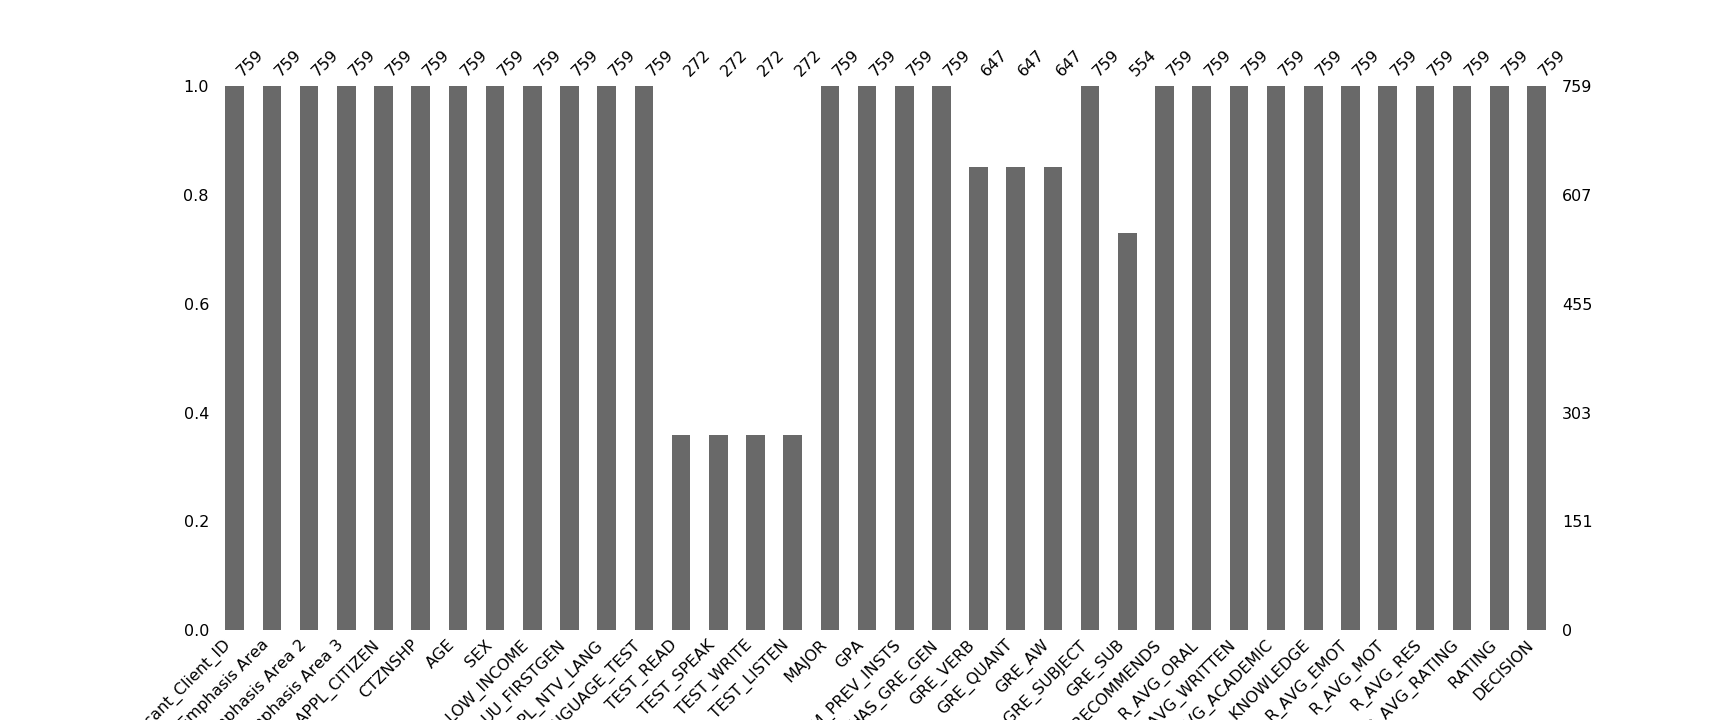
\includegraphics[width=11cm, height=5cm]{missing_data}
		\caption{Shorter columns shows the missing values.}
	\end{figure}		
\end{frame}
\begin{frame}{Data Visualization}
	\vspace{-2mm}
	%\frametitle{Credits}
	\begin{figure}
		%\caption{Learning rate too small}
		\centering
		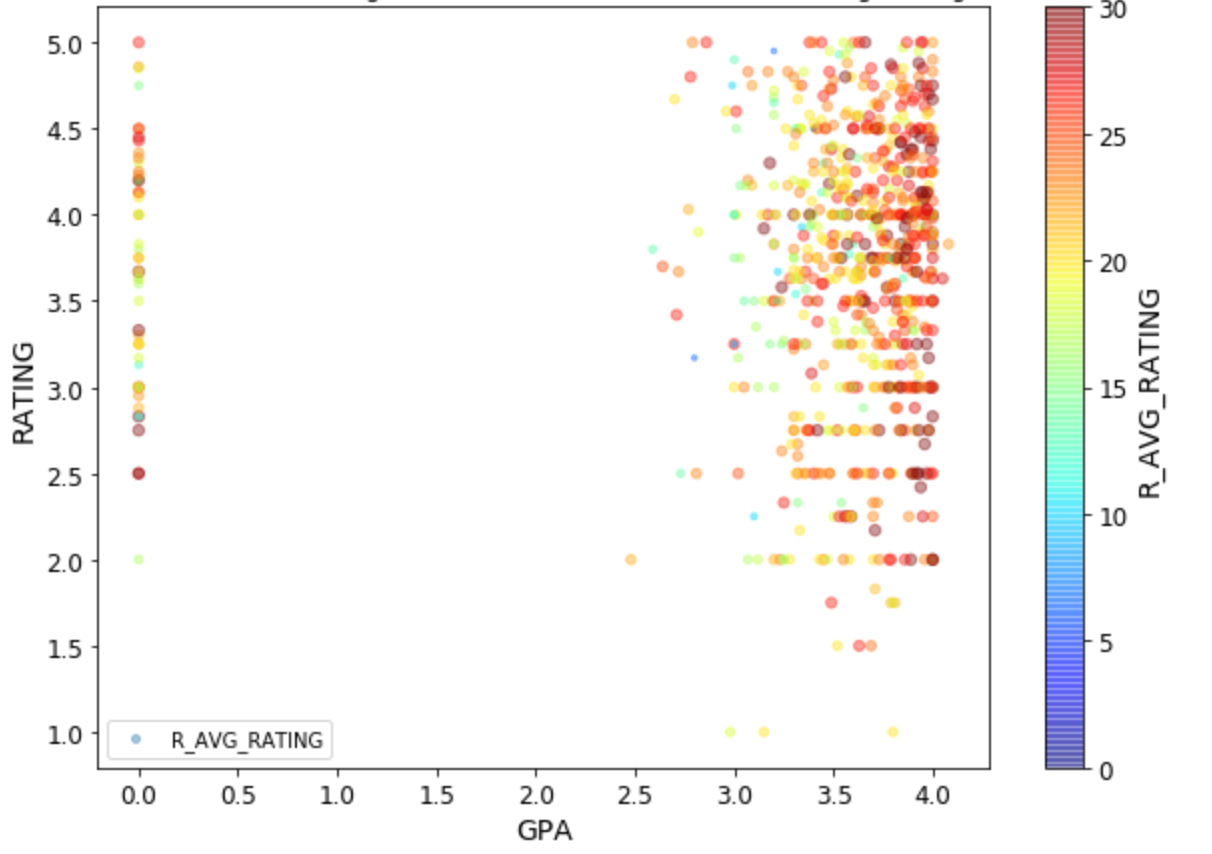
\includegraphics[width=11cm, height=6.5cm]{figure1a}
		\caption{The committee rating vs GPA based on recommenders' average rating}
	\end{figure}		
\end{frame}




\begin{frame}{Data Visualization}
	\vspace{-2mm}
	%\frametitle{Credits}
	\begin{figure}
		%\caption{Learning rate too small}
		\centering
		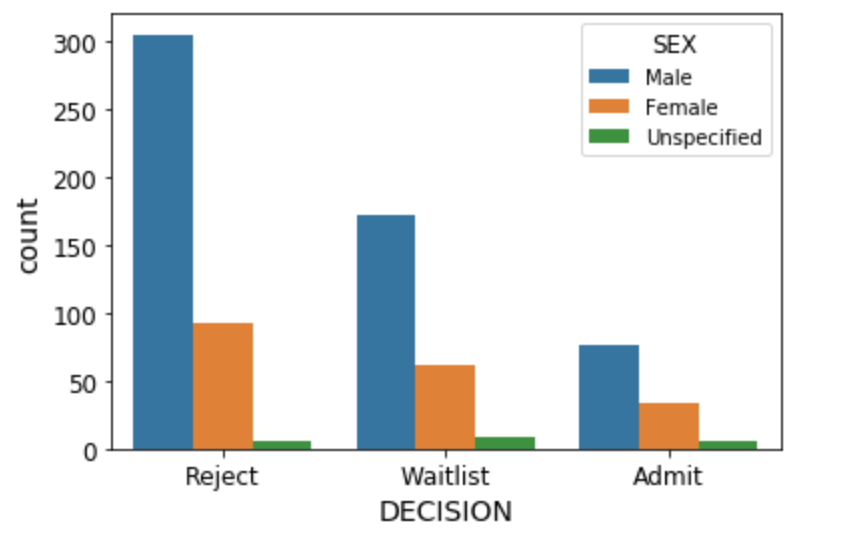
\includegraphics[width=11cm, height=6.5cm]{figure1b}
		%\caption{The committee rating vs GPA based on recommenders' average rating}
	\end{figure}		
\end{frame}

\begin{frame}{Data Visualization}
	\vspace{-2mm}
	%\frametitle{Credits}
	\begin{figure}
		%\caption{Learning rate too small}
		\centering
		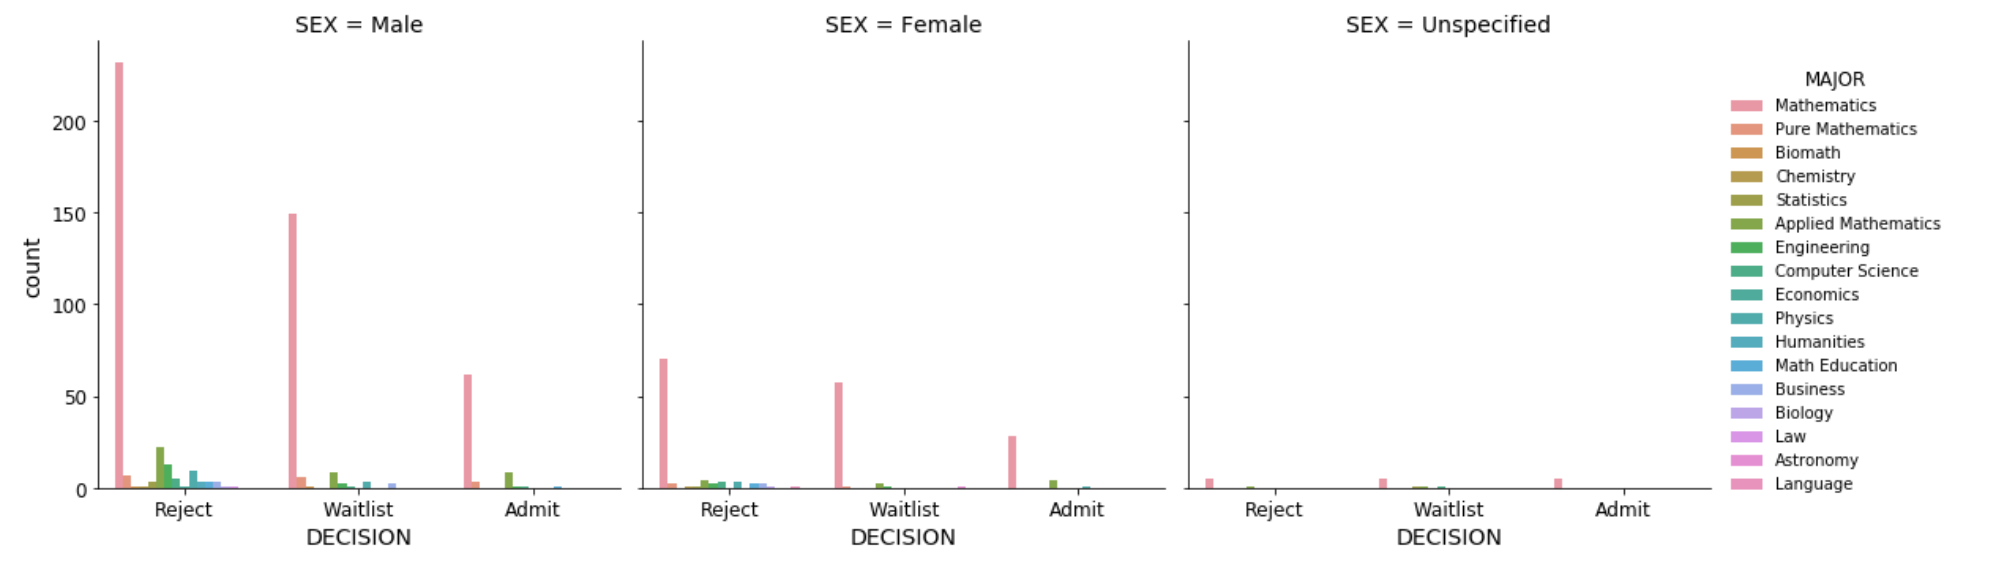
\includegraphics[width=10cm, height=5cm]{figure1c}
		%\caption{The committee rating vs GPA based on recommenders' average rating}
	\end{figure}		
\end{frame}

\begin{frame}{Data Visualization}
	\vspace{-2mm}
	%\frametitle{Credits}
	\begin{figure}
		%\caption{Learning rate too small}
		\centering
		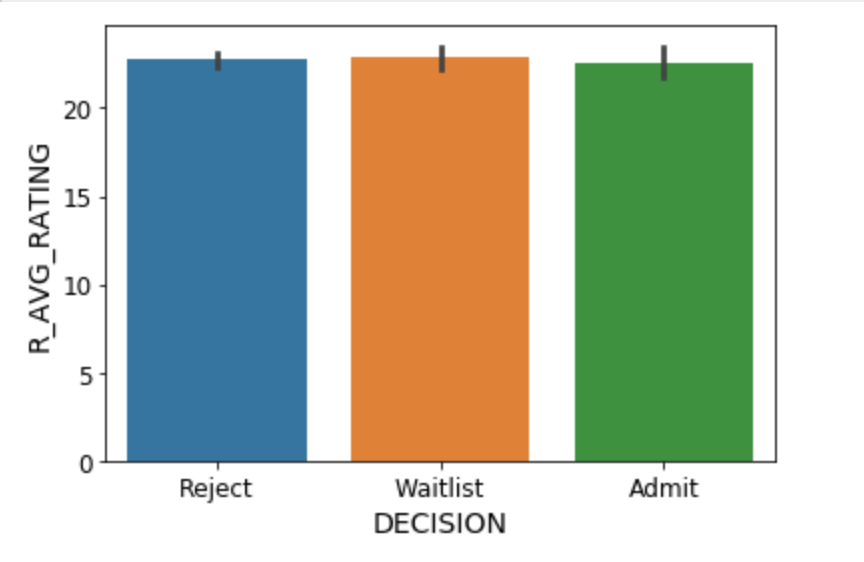
\includegraphics[width=11cm, height=6.5cm]{figure1d}
		%\caption{The committee rating vs GPA based on recommenders' average rating}
	\end{figure}		
\end{frame}

\begin{frame}{Data Visualization}
	\vspace{-2mm}
	%\frametitle{Credits}
	\begin{figure}
		%\caption{Learning rate too small}
		\centering
		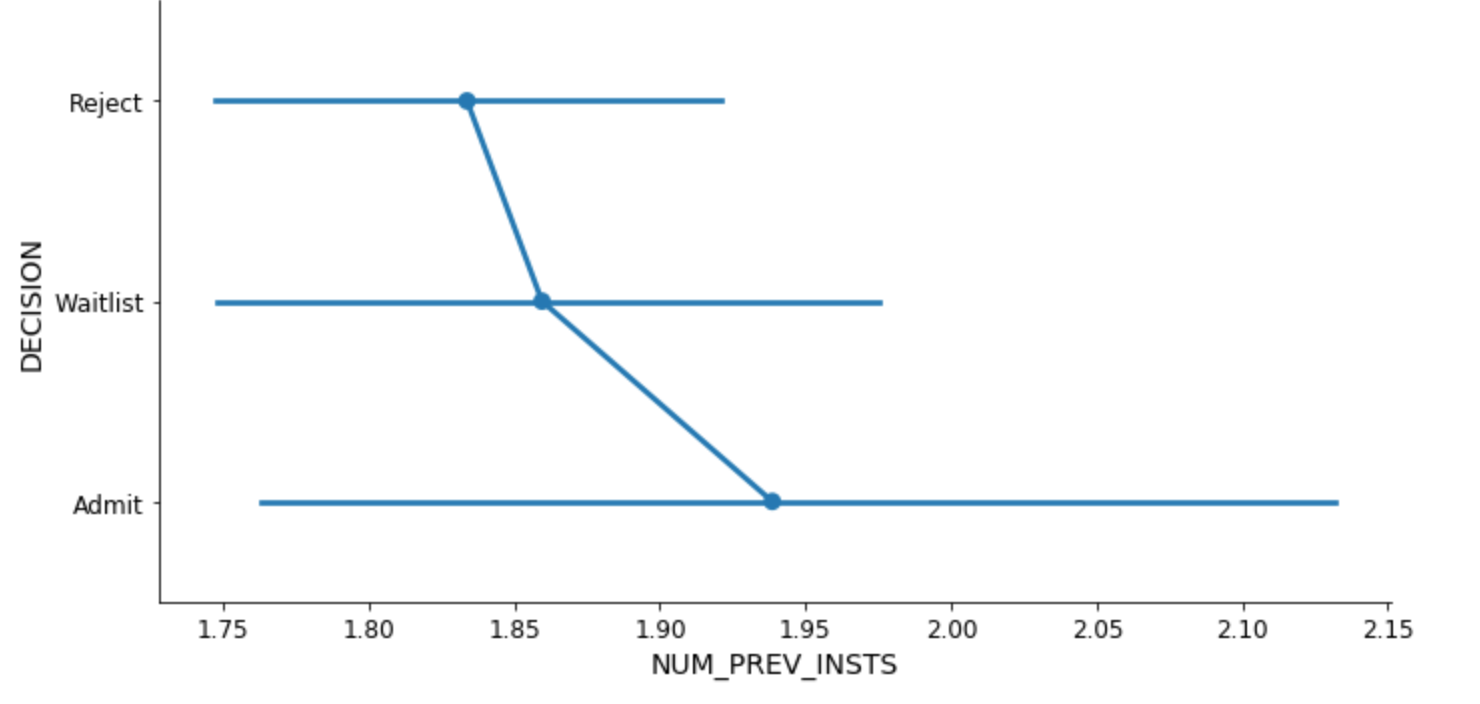
\includegraphics[width=11cm, height=6.5cm]{figure1e}
		%\caption{The committee rating vs GPA based on recommenders' average rating}
	\end{figure}		
\end{frame}
\section{Overview of the methods}

\begin{frame}
  \frametitle{Objectives}
\begin{itemize}
	\item Batch Gradient Descent
	\item Stochastic Gradient Descent
	\item Mini-Batch Gradient Descent
	%\pause
	%\item Gradient Boosting/XgBoost 
\pause	
	 \item Neural Networks
	 \pause
	  \item Stacking Approach
	 
	     %leave out the \pause on the final item
\end{itemize}
\end{frame}

\begin{frame}
	\frametitle{Gradient Descent}
	\begin{itemize}
		\item The general idea of Gradient Descent is to tweak parameters iteratively in order to minimize a cost function.
		\pause
		\item MSE cost function for a Linear Regression model
		 $$ MSE(X,\theta)=\frac{1}{m}\sum_{i=1}^m \left(\theta^T \cdot x^{(i)}-y^{(i)}\right)^2$$
		where  $\theta$ is the model’s parameter vector, containing the bias term $\theta_0$ and the feature
		weights $\theta_1$ to $\theta_n$.
		\item $x$ is the instance’s feature vector, containing $x_0$ to $x_n$, with $x_0$ always equal to 1. 
		%\item  $h_\theta$ is the hypothesis function, using the model parameters $\theta$.
		%\pause
		%leave out the \pause on the final item
	\end{itemize}
\end{frame}

\begin{frame}
	\frametitle{Gradient Descent}
	\begin{figure}
		%\caption{Learning rate too small}
		\centering
		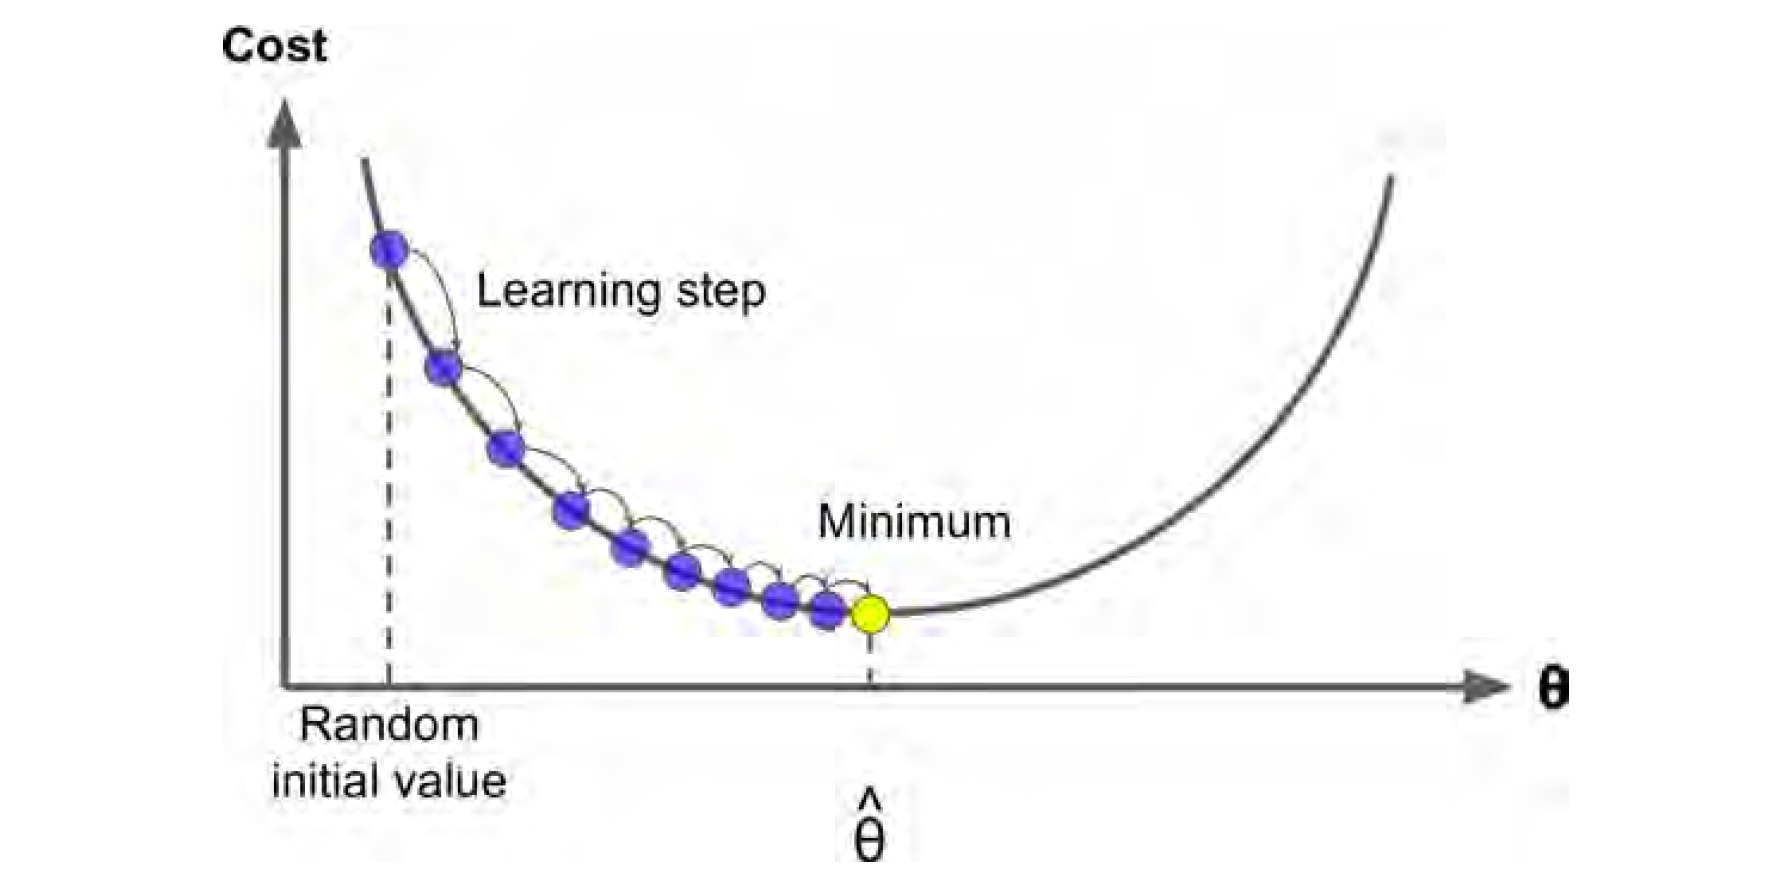
\includegraphics[scale=0.35]{figure4-3}
		\caption{Gradient Descent}
	\end{figure}		
	\end{frame}


\begin{frame}
	\frametitle{Gradient Descent}
	\begin{figure}
	%\caption{Learning rate too small}
	\centering
	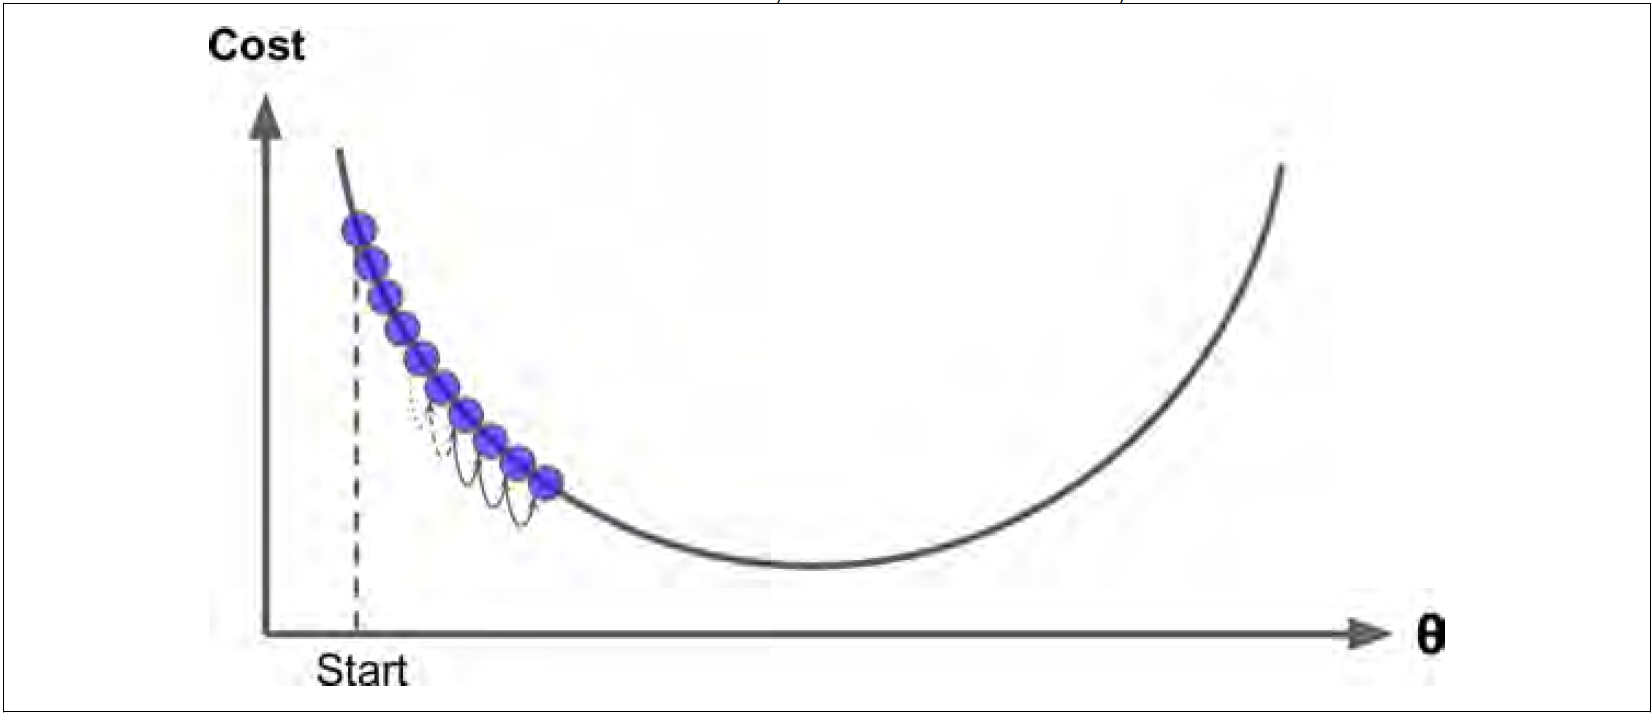
\includegraphics[scale=0.35]{figure4-4}
\caption{Learning rate too small}
	\end{figure}		
\end{frame}

\begin{frame}
	\frametitle{Gradient Descent}
	\begin{figure}
		%\caption{Learning rate too small}
		\centering
		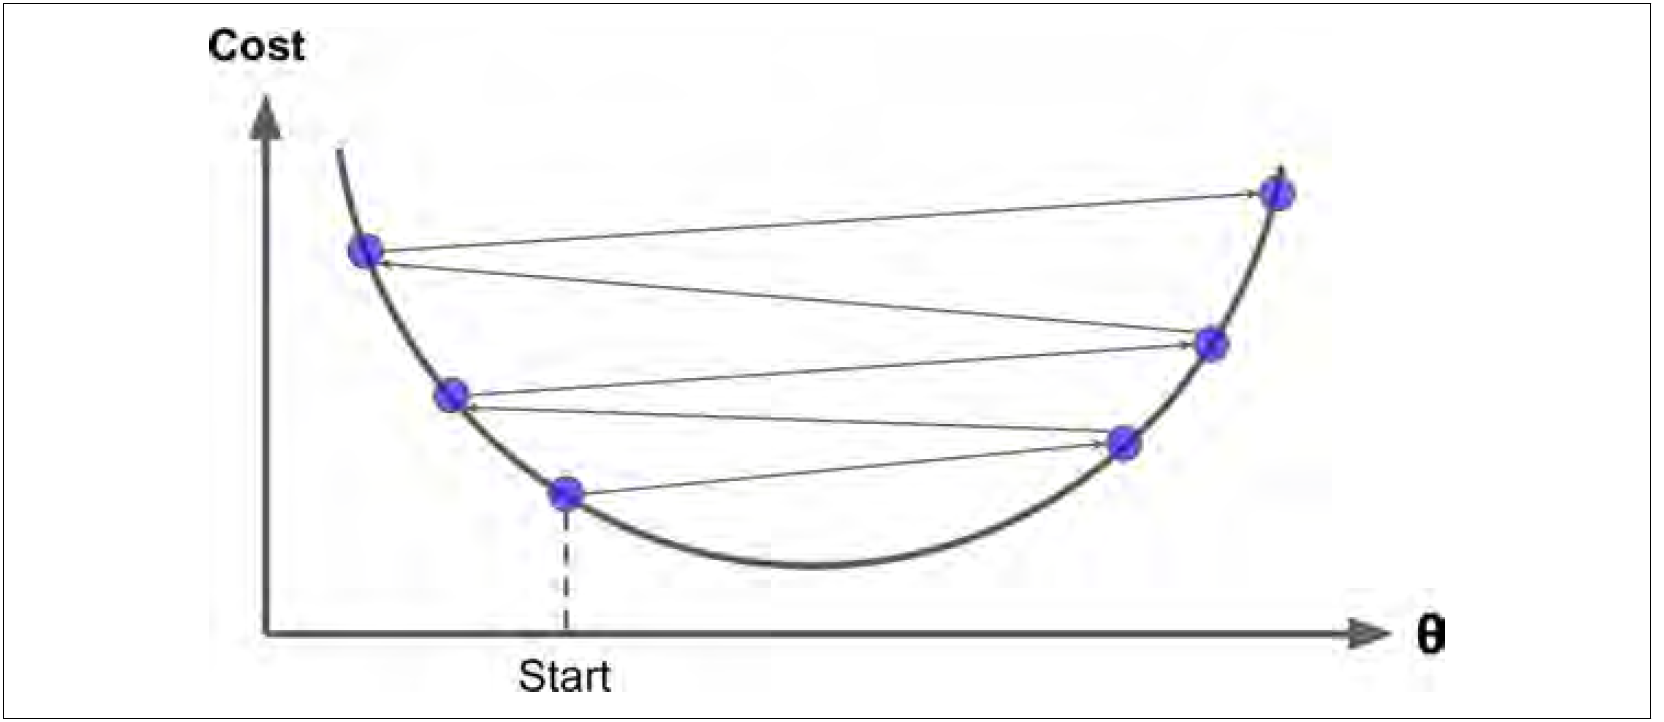
\includegraphics[scale=0.35]{figure4-5}
		\caption{Learning rate too large}
	\end{figure}		
\end{frame}


\begin{frame}
	\frametitle{Gradient Descent}
	\begin{figure}
		%\caption{Learning rate too small}
		\centering
		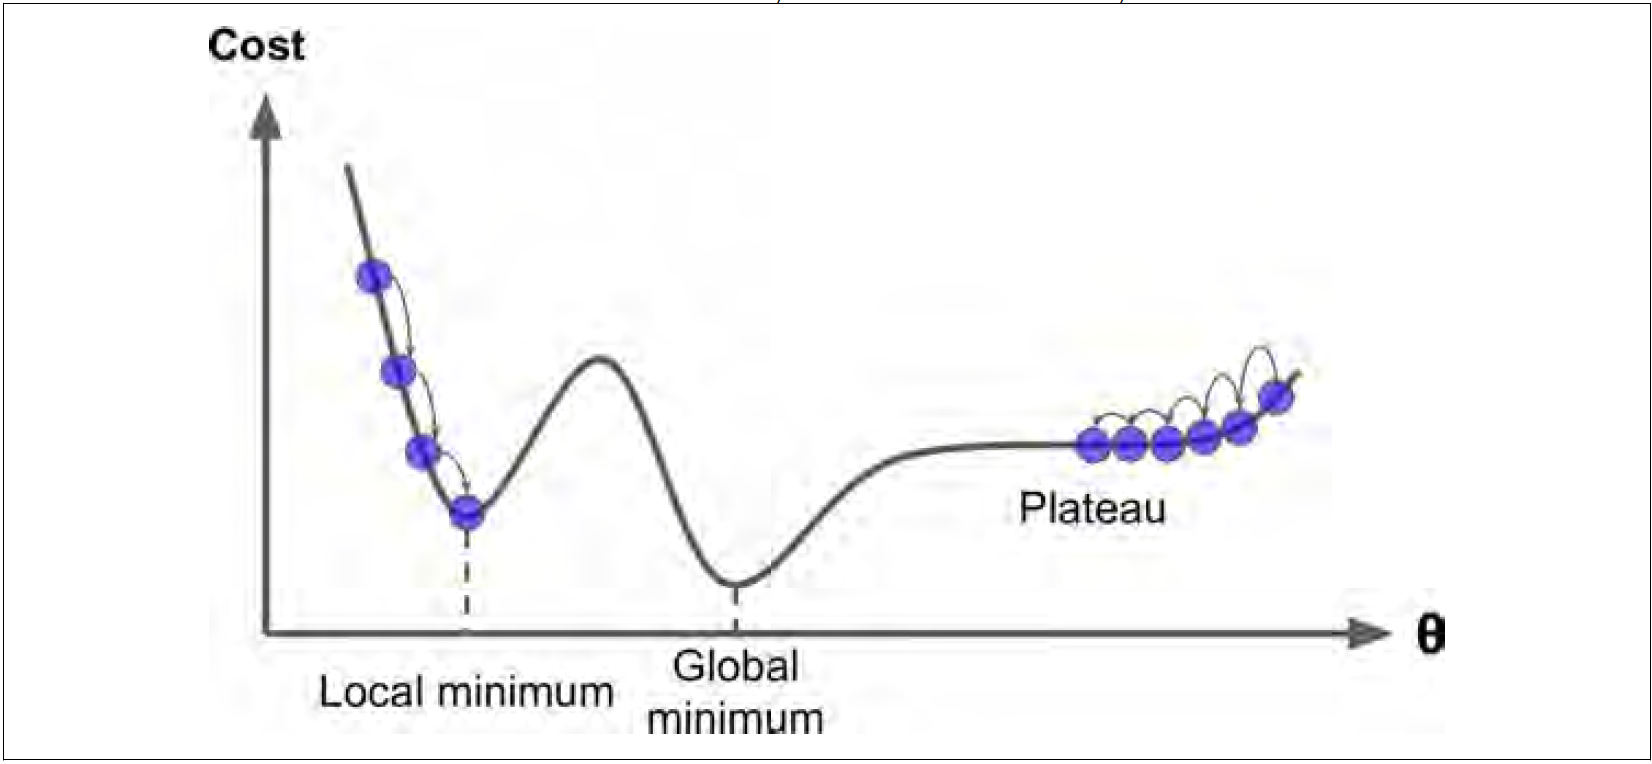
\includegraphics[scale=0.35]{figure4-6}
		\caption{Gradient Descent pitfalls}
	\end{figure}		
\end{frame}


\begin{frame}{Batch Gradient Descent}
%\frametitle{Credits}

To implement Gradient Descent, we need to compute the gradient of the cost function with regards to each model parameter $\theta_j$. In other words, we need to calculate partial derivatives 
$$\frac{\partial }{\partial \theta_j}MSE(\theta) = \frac{2}{m}\sum_{i=1}^m \left(\theta^T \cdot x^{(i)}-y^{(i)}\right)x^{(i)}_j.$$

Instead of computing these gradients individually, we can use 
$$ \nabla_\theta MSE(\theta)= \frac{2}{m}X^T\cdot(X\cdot \theta-y) $$
to compute them all in one go. The gradient vector, noted $\nabla_\theta MSE(\theta)$, contains all the partial derivatives of the cost function (one for each model parameter).
\end{frame}


\begin{frame}{Batch Gradient Descent}
	%\frametitle{Credits}
	
	Once you have the gradient vector, which points uphill, just go in the opposite direction to go downhill. This means subtracting $\nabla_\theta MSE(\theta)$ from $\theta$. This is where the learning rate $\eta$ comes into play: multiply the gradient vector by $\eta$ to determine the size of the downhill step.
	$$\theta^{next \; step }=\theta-\eta \nabla_\theta MSE(\theta).$$
	\pause
\begin{figure}
	%\caption{Learning rate too small}
	\centering
	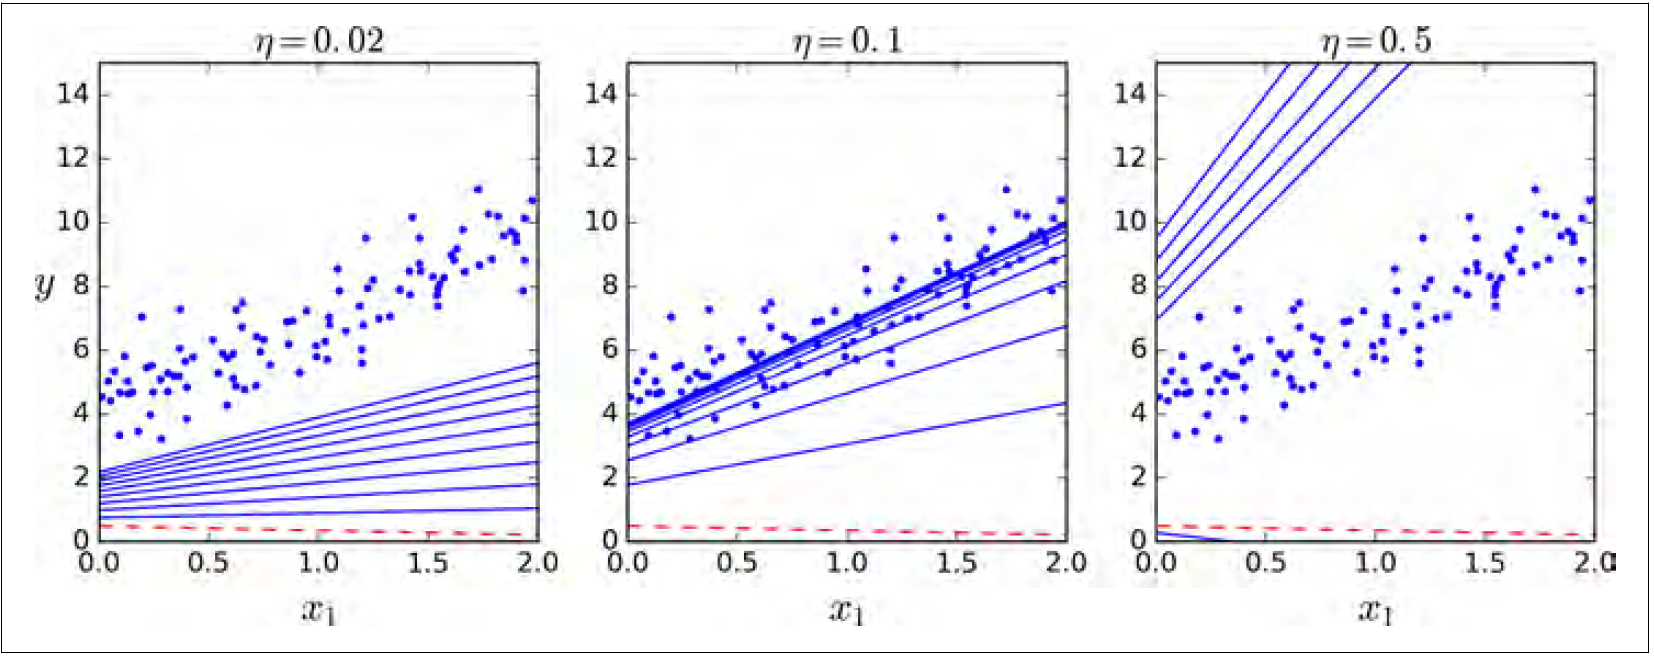
\includegraphics[scale=0.29]{figure4-8}
	\caption{Gradient Descent with various learning rates}
\end{figure}		
\end{frame}


\begin{frame}
	\frametitle{Stochastic Gradient Descent}
	\begin{itemize}
		\item The main problem with Batch Gradient Descent is the fact that it uses the whole training set to compute the gradients at every step, which makes it very slow when the training set is large. 
		\pause
		\item At the opposite extreme, Stochastic Gradient Descent just picks a random instance in the training set at every step and computes the gradients based only on that single instance.
		\begin{figure}
			%\caption{Learning rate too small}
			\centering
			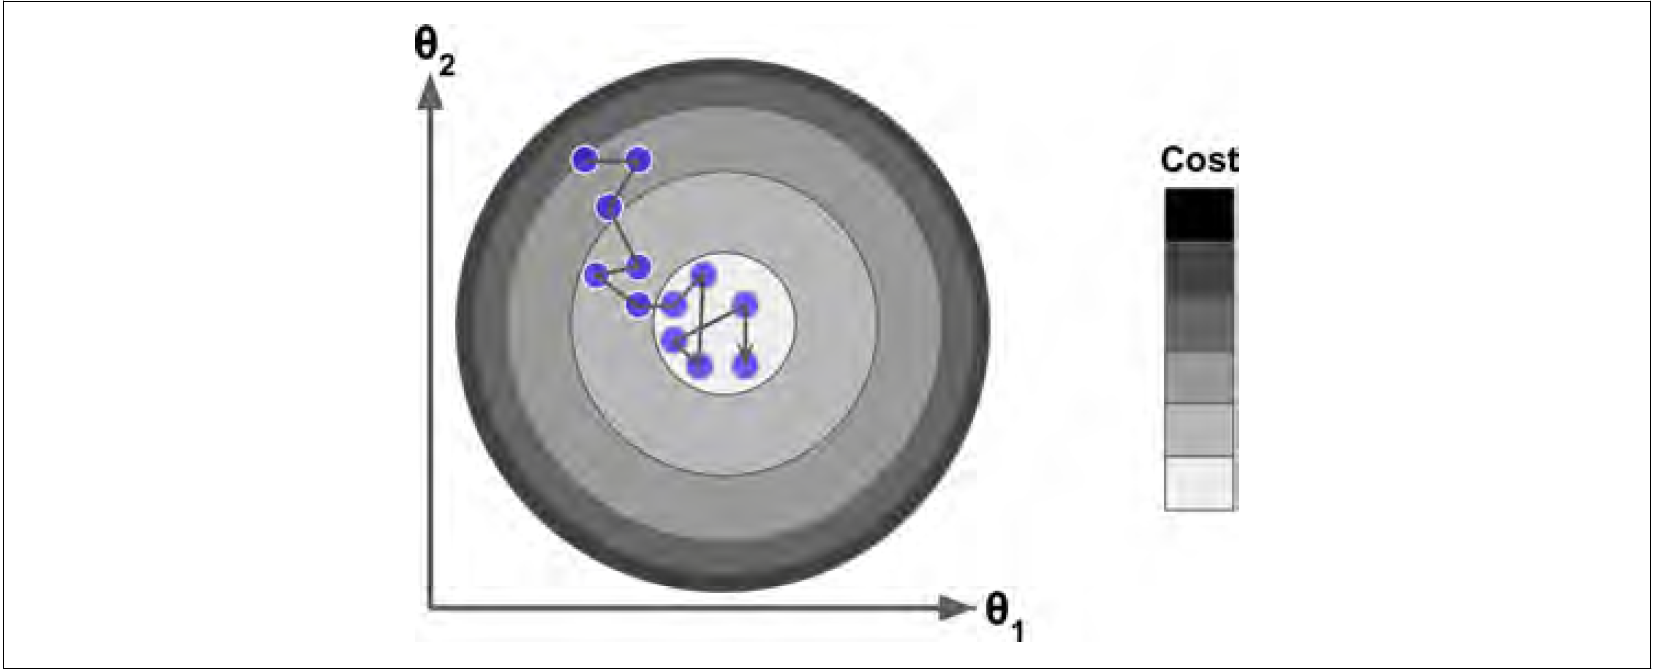
\includegraphics[scale=0.29]{figure4-9}
			\caption{Stochastic Gradient Descent}
		\end{figure}		
		%\item On the other hand, due to its stochastic (i.e., random) nature, this algorithm is much less regular than Batch Gradient Descent: instead of gently decreasing until it reaches the minimum, the cost function will bounce up and down, decreasing only on average.
		%\pause 
		%\item  $h_\theta$ is the hypothesis function, using the model parameters $\theta$.
		%\pause
		%leave out the \pause on the final item
	\end{itemize}
\end{frame}


\begin{frame}
	\frametitle{Mini-batch Gradient Descent}
	\begin{itemize}
		\item 
		 It is quite simple to understand once you know Batch and Stochastic Gradient Descent: at each step, instead of computing the gradients based on the full training set (as in Batch GD) or based on just one instance (as in Stochastic GD), Minibatch GD computes the gradients on small random sets of instances called minibatches.
		\begin{figure}
			%\caption{Learning rate too small}
			\centering
			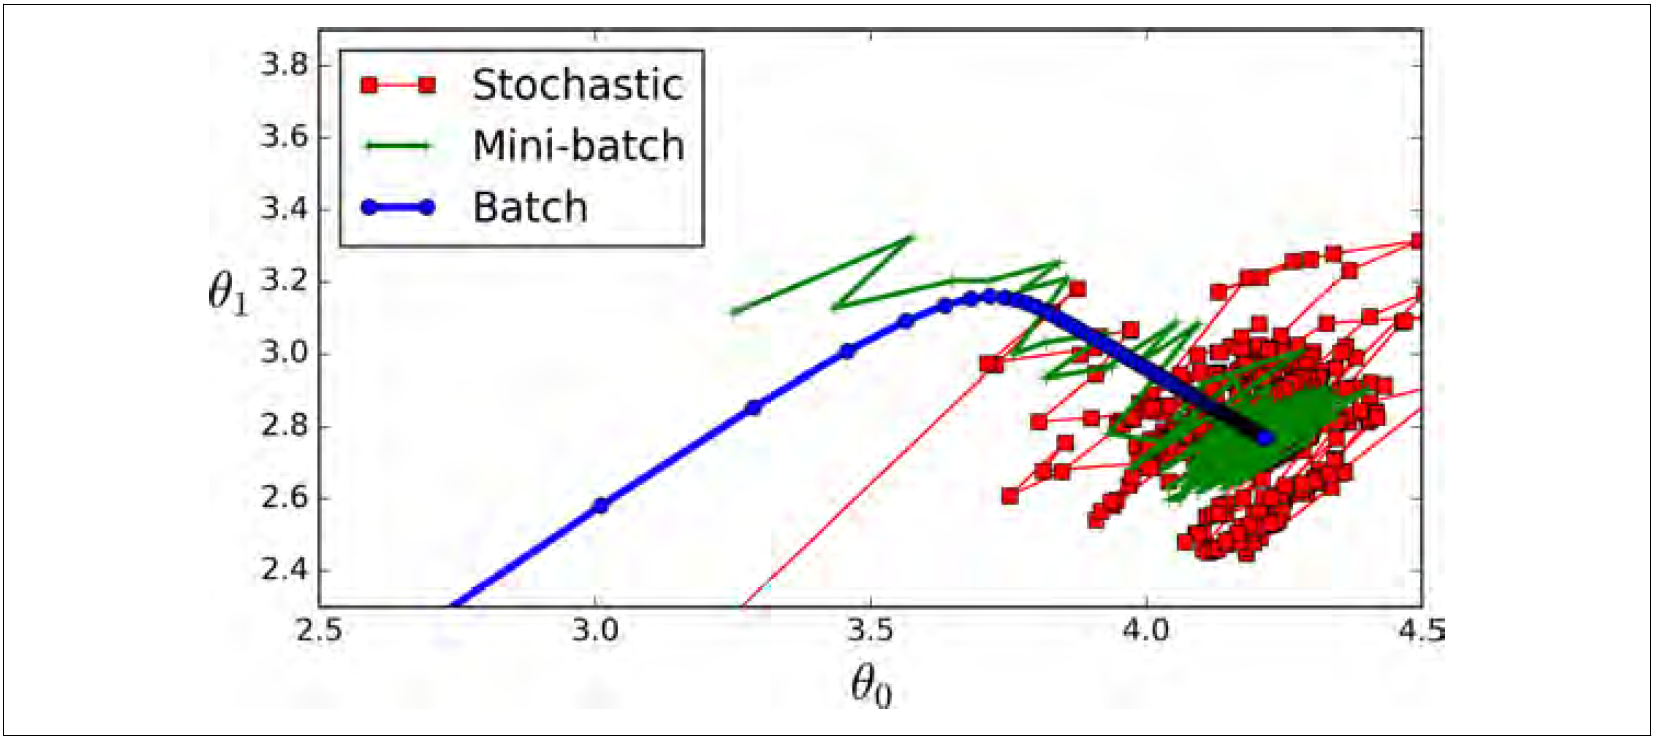
\includegraphics[scale=0.29]{figure4-11}
			\caption{Gradient Descent paths in parameter space}
		\end{figure}		
		%\pause
		%leave out the \pause on the final item
	\end{itemize}
\end{frame}

%\begin{frame}
%\frametitle{Histograms of Coin  Toss}
%	\centering
%\includegraphics[scale=0.34]{Figure1.png}

%\end{frame}

\begin{frame}{Neural Networks}
\framesubtitle{Building Blocks: Neurons}

	\begin{figure}
	%\caption{Learning rate too small}
	\centering
	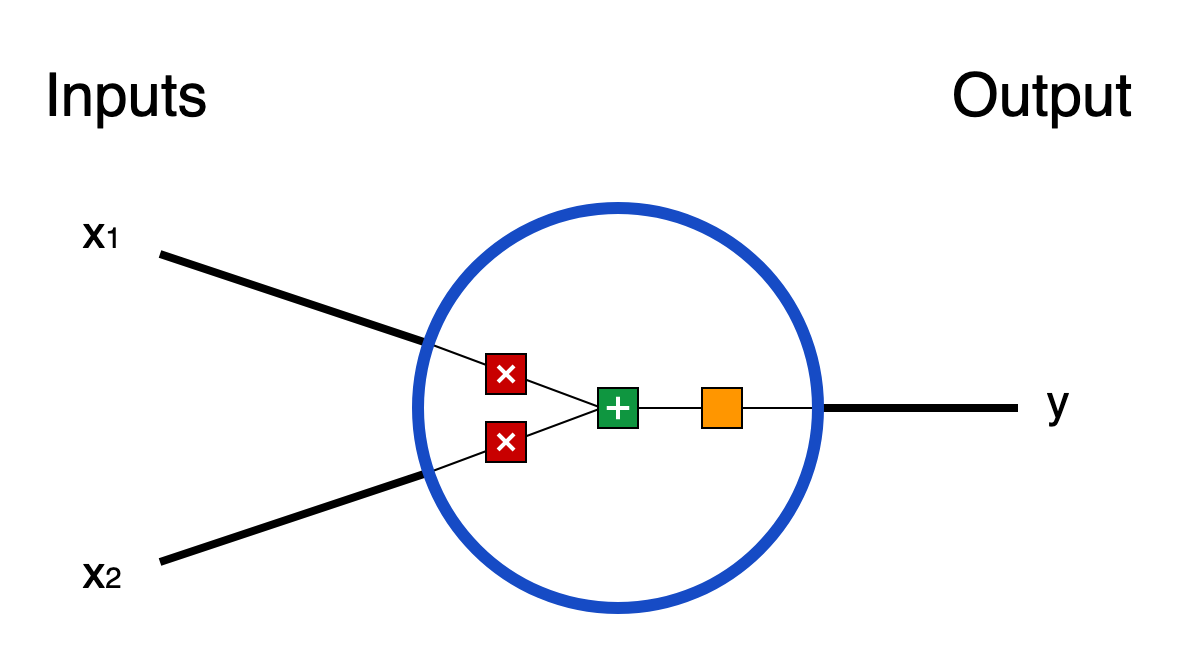
\includegraphics[scale=0.49]{twoinputneurons}
	\caption{Single neuron with 2 inputs}
\end{figure}		
\end{frame}
%
%\begin{frame}
%\frametitle{Simulation of  RWRP}
%\begin{center}
%	\movie[height=5cm,width=6.5cm,poster,autostart,loop]{}{leaves.avi}
%\end{center}
%\begin{itemize}
%	\item Movies only seem to work in Adobe Reader
%	\item Movie file is not embedded, it must be on the computer
%\end{itemize}
%\end{frame}

\begin{frame}{Activation function}
%\frametitle{Credits}



	  The activation function is used to turn an unbounded input into an output that has a nice, predictable form. A commonly used activation function is the sigmoid function:
	\begin{equation*}
	 S(x)={\frac {1}{1+e^{-x}}}={\frac {e^{x}}{e^{x}+1}}.
	\end{equation*}

		\begin{figure}
		%\caption{Learning rate too small}
		\centering
		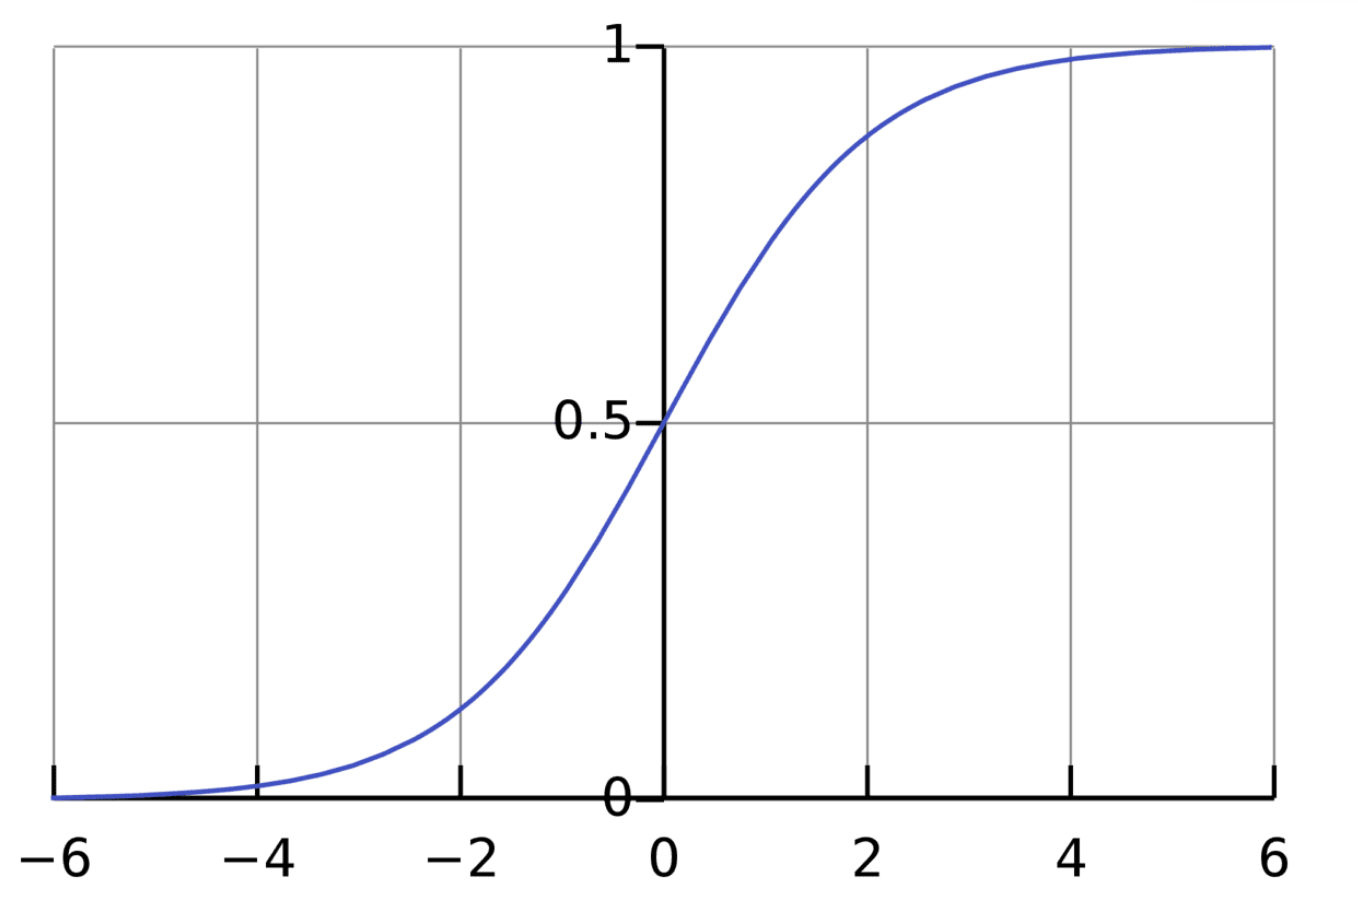
\includegraphics[scale=0.29]{sigmoid}
		\caption{Sigmoid function}
	\end{figure}		
	
\end{frame}

\begin{frame}{Combining Neurons into a Neural Network}
%\frametitle{Credits}
	\begin{figure}
	%\caption{Learning rate too small}
	\centering
	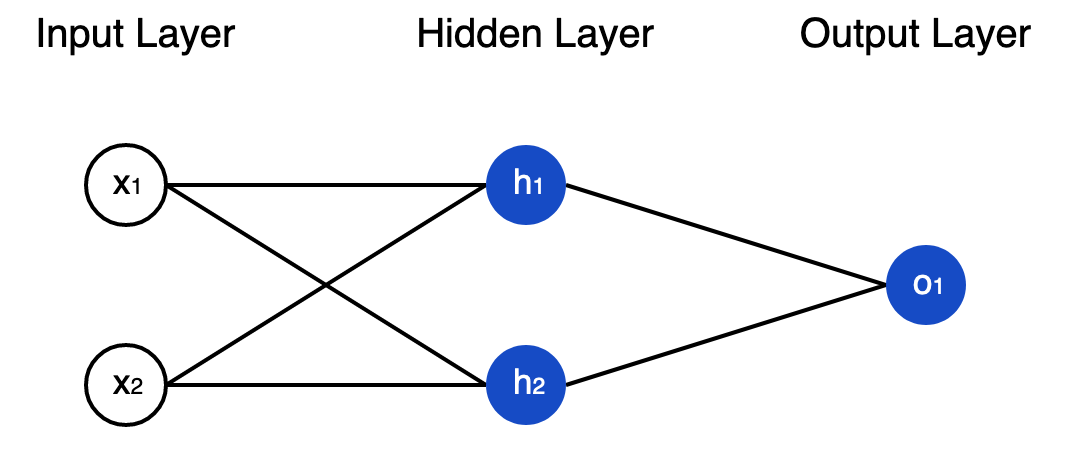
\includegraphics[scale=0.49]{neuralnetwork}
	\caption{Neural Network with 2 inputs, 1 hidden layer with 2 neurons ($h_1$ and $h_2$) and 1 output neuron $o_1$ }
\end{figure}		
\end{frame}

\begin{frame}{Training a Neural Network}
%\frametitle{Credits}
\begin{itemize}
	\item  Training network to predict someone’s gender given their weight and height:
	
	\begin{figure}
		%\caption{Learning rate too small}
		\centering
		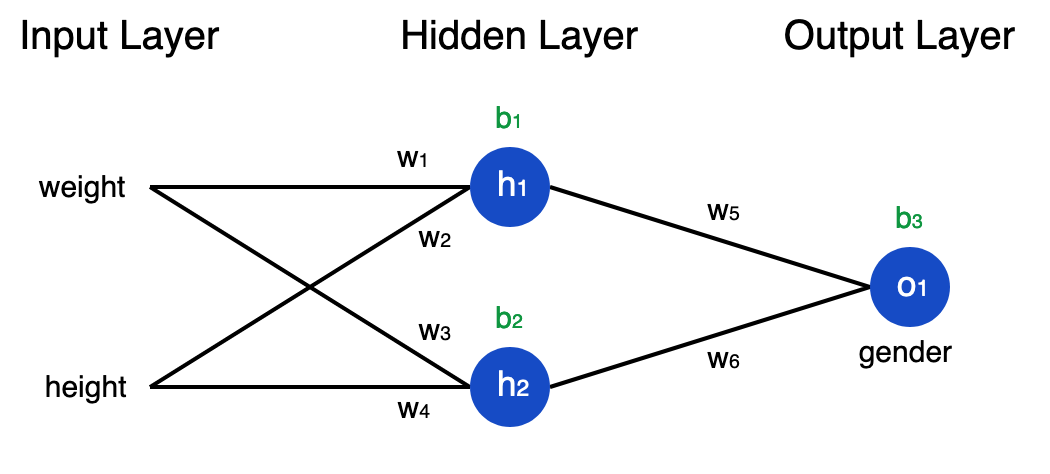
\includegraphics[scale=0.49]{neuralnetworktraning2}
	\end{figure}		
		\item Then, we can write loss as a multivariable function:
	$$L(w_1,w_2,w_3,w_4,w_5,w_6,b_1,b_2,b_3)$$
	
\end{itemize}
\end{frame}

\begin{frame}{Back Propagation}
\vspace{-2mm}
%\frametitle{Credits}
\begin{itemize}
	\item  How would loss $L$ change if we changed $w_1$? That's a question the partial derivative $\frac{\partial L}{\partial w_1}$ can answer. 
	\pause 
	 $$\dfrac{\partial L}{\partial w_1}= \dfrac{\partial L}{\partial y_{pred}}*\dfrac{\partial y_{pred}}{\partial w_1} .$$
	\pause 
	\item Recall $ y_{pred}=o_1=f(w_5*h_1+w_6*h_2+b_3)$.
	\pause 
	$$\dfrac{\partial y_{pred}}{\partial w_1} =\dfrac{\partial y_{pred}}{\partial h_1} *\dfrac{\partial h_1}{\partial w_1} .$$
	\item Also recall $h_1 = f(w_1x_1+w_2x_2+b_1)$. Finally we get
	\pause 
	$$\dfrac{\partial L}{\partial w_1} = \dfrac{\partial L}{\partial y_{pred}}*\dfrac{\partial y_{pred}}{\partial h_1}*\dfrac{\partial h_1}{\partial w_1}.$$
\end{itemize}
\end{frame}

%\begin{frame}
%\frametitle{Picture }
%\begin{figure}
%\centering
%	\includegraphics[width=3cm]{lion.png}
%\end{figure}
%\end{frame}

\begin{frame}{Algorithm} 
%\frametitle{Credits}
\vspace{-2mm}
\begin{itemize}
	\item  Update equation
	
	\[w_1\leftarrow w_1-\eta \dfrac{\partial L}{\partial w_1}\] 
	
	$\eta$ is a constant called the learning rate that controls how fast we train. All we're doing is subtracting $\eta \frac{\partial L}{\partial w_1}$ from $w_1$:
	\pause 
	\item If $\frac{\partial L}{\partial w_1}$ is positive, $w_1$ will decrease, which makes $L$ decrease.
	\pause 
	\item  If $\frac{\partial L}{\partial w_1}$ is negative, $w_1$ will increase, which makes $L$ decrease.
	\end{itemize}
\end{frame}
%
%\begin{frame}
%\frametitle{Picture }
%\begin{figure}
%	\centering
%	\includegraphics[width=3cm]{lion.png}
%\end{figure}
%\end{frame}



\begin{frame}{Stacking Approach}
	%\frametitle{Credits}
	\begin{itemize}
		\item Suppose we have trained a few classifiers, each one achieving about 80\% accuracy.
		\pause 
\item  A Logistic Regression classifier, an SVM classifier, a Random Forest classifier, a K-Nearest Neighbors classifier, and perhaps a few more
	\end{itemize}
\begin{figure}
	%\caption{Learning rate too small}
	\centering
	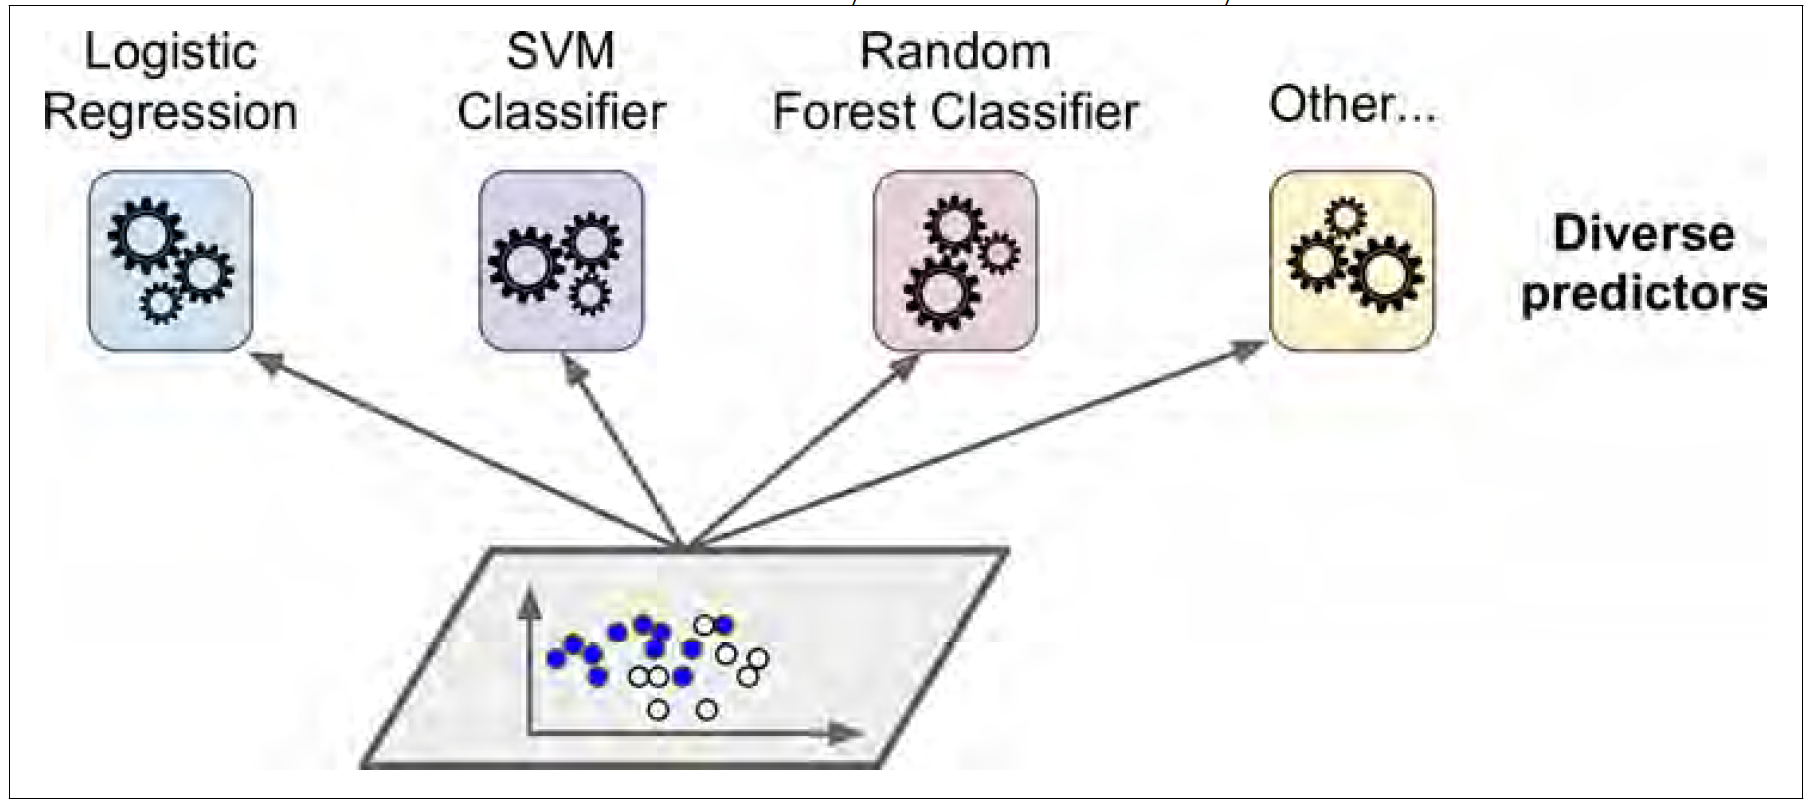
\includegraphics[scale=0.29]{figure7-1}
	\caption{Training diverse classifiers}
\end{figure}		
\end{frame}

\begin{frame}{Stacking Approach}
	%\frametitle{Credits}
	\begin{itemize}
		\item A very simple way to create an even better classifier is to aggregate the predictions of each classifier and predict the class that gets the most votes. 
		\pause
		\item This majority-vote classifier is called a \textbf{hard voting} classifier.
	\end{itemize}
	\begin{figure}
		%\caption{Learning rate too small}
		\centering
		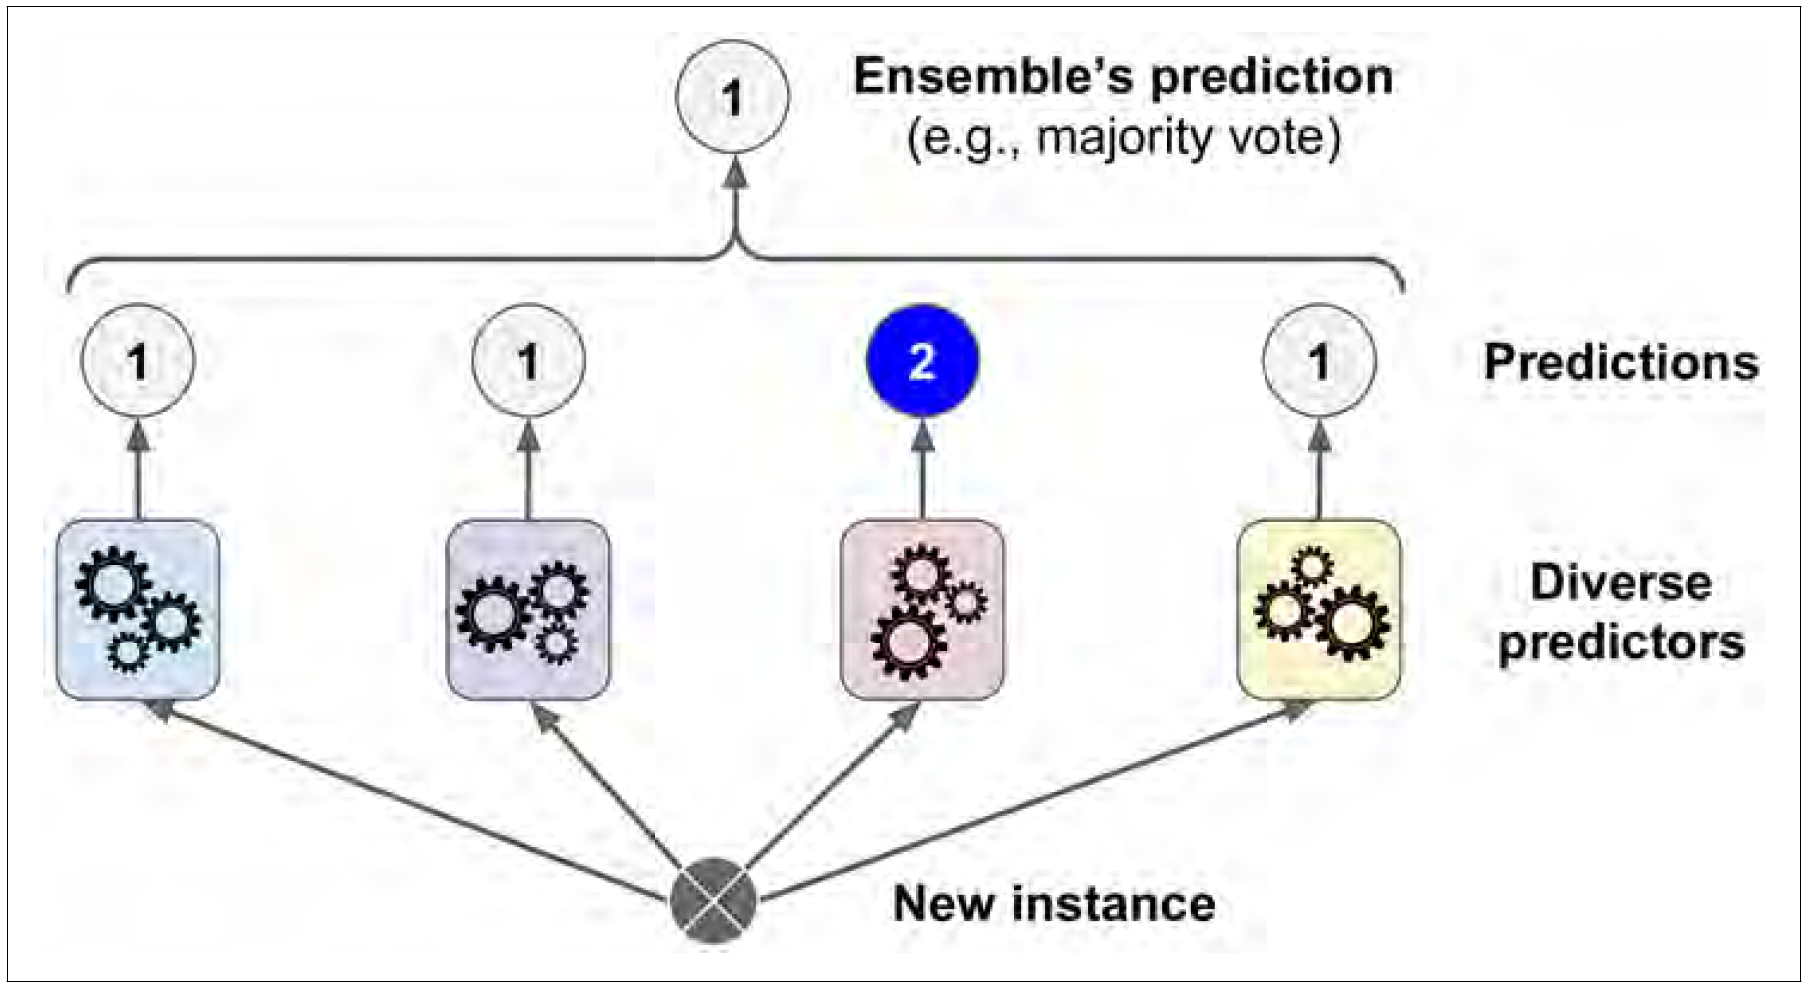
\includegraphics[scale=0.29]{figure7-2}
		\caption{Hard voting classifier predictions}
	\end{figure}		
\end{frame}

\begin{frame}{Results for predicting the Decision}
	
\begin{figure}
	\centering
	\begin{minipage}{0.49\textwidth}
		\centering
		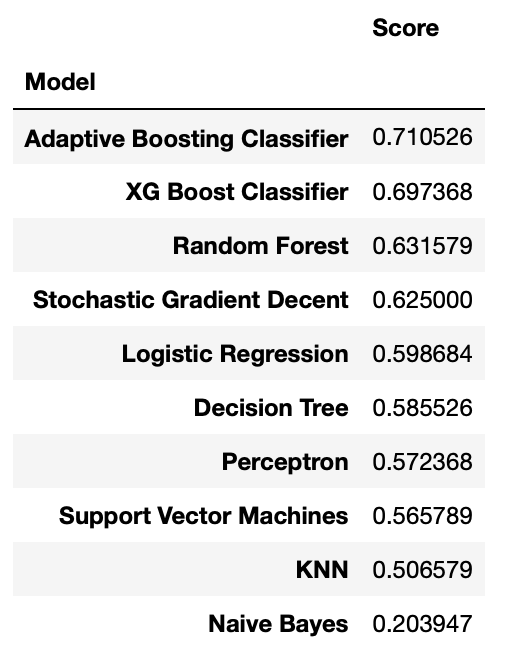
\includegraphics[width=1\textwidth]{Table1Decision} % first figure itself
		\caption{Default Parameters of the models}
	\end{minipage}\hfill
	\begin{minipage}{0.49\textwidth}
		\centering
		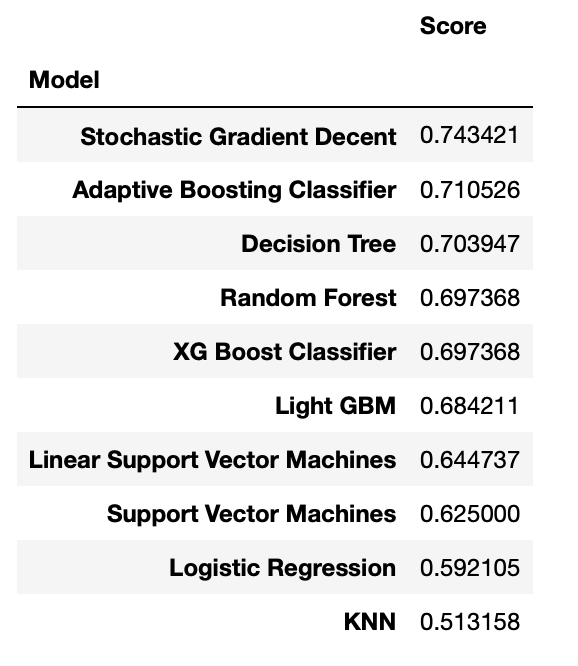
\includegraphics[width=1\textwidth]{Table2Decision} % second figure itself
		\caption{Models with Grid Search}
	\end{minipage}
\end{figure}
\end{frame}

\section{Results}
\begin{frame}{Results for predicting the Decision}
\framesubtitle{ Stacking approach and h2o AutoML results}
\begin{itemize}
	\item For stacking approach:
	average accuracy on a train set: 0.840197
	\pause 
	\item For stacking approach:
average accuracy on a test set: 0.703947
\pause 
\item For h2o AutoML:
average accuracy on a train set: 0.793297
	\pause 
	\item For h2o AutoML:
	average accuracy on a test set: 0.703947
	\end{itemize}
\end{frame}
%\begin{frame}
%\begin{itemize}
%	\item Let $\range=\lbrace e_1,e_2\rbrace$. Add picture. here
%\end{itemize}
%\end{frame}


\begin{frame}{Conclusion about predicting the decision variable}
\begin{figure}
	%\caption{Learning rate too small}
	\centering
	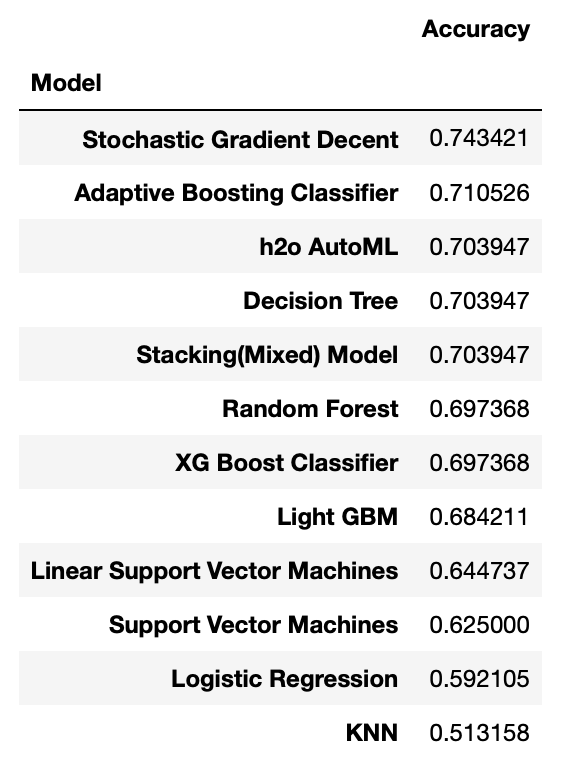
\includegraphics[scale =0.50]{TableDecisionConclusion}
	%\caption{The committee rating vs GPA based on recommenders' average rating}
\end{figure}		
\end{frame}


\begin{frame}
\frametitle{Estimating the RATING variable}
\begin{figure}
	%\caption{Learning rate too small}
	\centering
	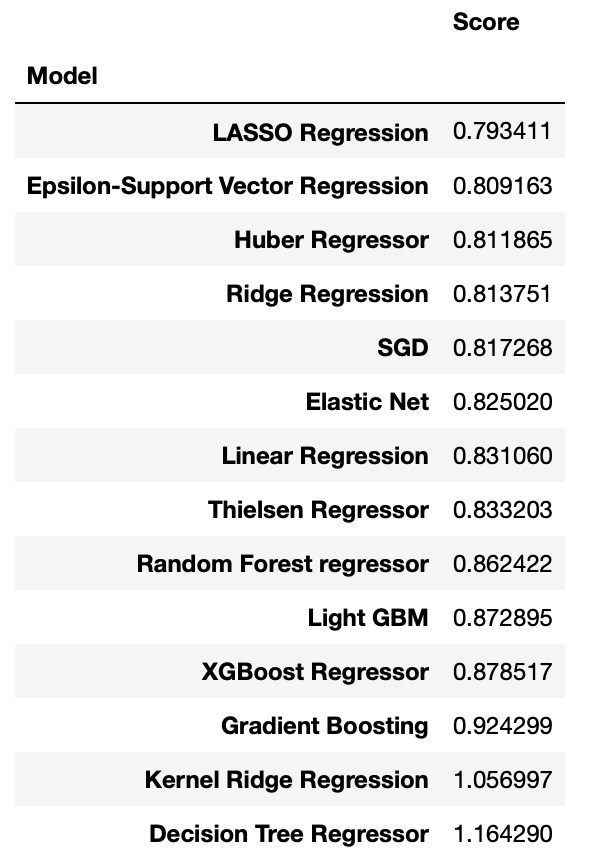
\includegraphics[scale =0.45]{Table1Rating}
	\caption{These results are on a train set}
\end{figure}		
\end{frame}

\begin{frame}{Results for predicting the Rating}
	\framesubtitle{ Stacking approach and h2o AutoML results}
	\begin{itemize}
		\item For stacking approach:
		RMSE score on a train data: 0.791428
		\pause 
		\item For stacking approach:
		RMSE score on a test data: 0.811798
		\pause 
		\item For h2o AutoML:
		RMSE score on a train data:  0.770774
		\pause 
		\item For h2o AutoML:
		RMSE score on a test data: 0.840311
	\end{itemize}
\end{frame}

\begin{frame}{Results for predicting the Rating}
	\framesubtitle{ Using other h2o models}
	\begin{itemize}
		\item For GBM:
		RMSE score on a train data: 0.679267
		\pause 
			\item For GBM:
		RMSE score on a test data: 0.838749
		\pause 
		\item For RF:
		RMSE score on a train data: 0.735665
		\pause 
		\item For RF:
		RMSE score on a test data: 0.838040
		\pause 
		\item For deep learning with 3 hidden layers and 128 neurons:
		RMSE score on a train data: 0.573881
		\pause 
		\item For deep learning with 3 hidden layers and 128 neurons:
		RMSE score on a test data: 0.895573
	\end{itemize}
\end{frame}

\begin{frame}{Conclusion about predicting the Rating variable}
	\begin{figure}
		%\caption{Learning rate too small}
		\centering
		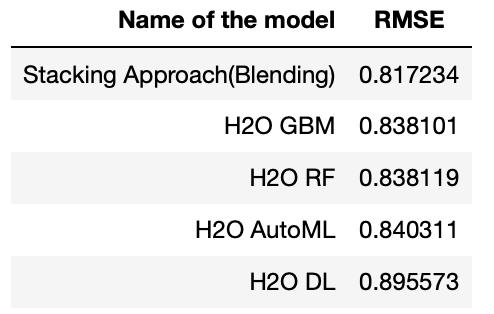
\includegraphics[scale =0.50]{TableRatingConclusion}
		\caption{RMSE scores}
	\end{figure}		
\end{frame}

\begin{frame}
\frametitle{Conclusion}

\begin{itemize}
	\item The results of this analysis point to a common choice of the most relevant predictor variables:
	\begin{itemize}
		\item Applicant's age
		\item Applicant's GPA
		\item Applicant's choice of emphasis area for study in graduate school
		\item Applicant's GRE scores
		\item Applicant's undergraduate major
		\item Applicant's average ratings of knowledge given by applicant's recommenders
		\end{itemize} 
	\item In both cases, predicting the decision and predicting the rating variable, we see that some simpler models gave us better result comparing to more complicated models. One possible explanation of this could be the relationship between our variables and the response is linear. Another explanation would be the number of sample is not too many.
\end{itemize}
\end{frame}

\begin{frame}
\frametitle{Further Comments}

\begin{itemize}
\item For the future work, one might try multiple imputation technique instead of basic method to fill the missing values.
\pause 
\item There can be extra variables that represent the number of publications, and where they are published and impact factor of journals.

\pause
\item Having distributions of the GPA's of the universities where students are coming from may lead to have better prediction of the decision about students.
\pause
\item  It would also be useful to have a quantative opinion of the strength of  each recommender. 

\end{itemize}
\end{frame}


\begin{frame}
	\centering \Huge
	Thank you!
\end{frame}


\end{document}